\documentclass[11pt,spanish]{article} % Tipo y tamaño de letra del documento.

\usepackage{verbatim}
\usepackage[utf8]{inputenc}
\usepackage{subfiles}
\usepackage{biblatex}
\addbibresource{references.bib}
\usepackage{multicol}
\usepackage{amsfonts}
\usepackage{blindtext}
\usepackage{mathrsfs}
\usepackage{amsmath}
\usepackage{siunitx}
\usepackage{centernot}
\usepackage[shortlabels]{enumitem}
\usepackage{subfig}
\usepackage{datetime}
\usepackage{listingsutf8}
\usepackage[spanish]{babel}
\usepackage{tikz}
\usepackage{hyperref}
\usepackage[vlined,ruled,linesnumbered]{algorithm2e}
\usepackage{listings}
\usepackage{float}
\usepackage{url}
\usepackage{csquotes}
\usepackage{fourier} %font
\usepackage[top=2cm, bottom=2cm, left=2.5cm, right=2.5cm]{geometry}
\usepackage{pgfplots}
\usepackage{fancyhdr}
\usepackage{mdframed}
\usepackage{tikzducks}
\usepackage[nameinlink]{cleveref}
\usepackage{epigraph} 

\pgfplotsset{compat=1.18}

\usetikzlibrary{shapes.arrows, shapes.geometric, arrows.meta,angles,quotes,positioning,arrows,fit,quotes,calc}
\tikzset{>=latex} 

\setlength\algomargin{1em} 
\SetFuncSty{sc} 
\SetCommentSty{em} 


\Crefname{figure}{Fig.}{Figs.}
\newcommand\crefrangeconjunction{--}
\Crefname{table}{Tabla}{Tablas}
\Crefname{subsubsection}{Subsubsec.}{Subsubsections}
\Crefname{subsection}{Subsec.}{Subsections}
\Crefname{section}{Sec.}{Sections}
\Crefname{equation}{eq.}{eqs.}
\crefname{thm}{Theorem}{theorems}
\Crefname{thm}{Theorem}{Theorems} 

\definecolor{algoco}{rgb}{0,0.4,1}

\hypersetup{
  colorlinks=true,
  linkcolor=algoco,
  citecolor=blue,
  urlcolor=blue,
}

\lstset{
extendedchars=true
inputencoding=utf8/latin1,
basicstyle=\footnotesize\sffamily\color{black},
commentstyle=\slshape \color{gray},
numbers=left,
numbersep=10pt,
numberstyle=\tiny\color{red!80!black},
keywordstyle=\color{red!80!magenta},
showspaces=false,
showstringspaces=false,
stringstyle=\color{cyan!80!black},
tabsize=2,
literate={á}{{\'a}}1 {é}{{\'e}}1 {í}{{\'i}}1 {ó}{{\'o}}1 {ú}{{\'u}}1,
frame = single, 
numbers = none,
float, floatplacement = ht, captionpos = b,
xleftmargin = 2em, xrightmargin = 2em, 
}

\newcommand{\ub}[1]{\underbrace{#1}}
\newcommand\tcm{\textcolor{magenta}}
\newcommand\tca{\textcolor{algoco}}

\setlength\epigraphwidth{.7\textwidth} 

\newcommand{\tnum}{2 y 3} % reemplace 2 por el número de la tarea
\newcommand{\sem}{2024-2} % reemplace 2024-2 por el semestre correspondiente
\newcommand{\campus}{San Joaquín \\ Santiago} % reemplace Casa Central por el campus correspondiente
\newcommand{\rolusm}{202173564-k} % reemplace 2025073100-1 por su rol
\newcommand{\namestudent}{Carlos Vera Quezada} % reemplace Al Goritmo Pérez por su nombre

\headheight=14pt
\linespread{1.3}
\author{\namestudent}
\pagestyle{fancy}
\fancyhf{}%
\fancyfoot[R]{ \namestudent \\ \rolusm}
\fancyfoot[L]{Campus \campus} 
\fancyfoot[C]{\thepage}
\rhead{2024-2}
\lhead{INF-221}
\renewcommand{\headrulewidth}{0.4pt}
\renewcommand{\footrulewidth}{0.4pt}
\newbool{programs}
\boolfalse{programs}
\chead{REPORTE TAREA \tnum~}



\title{
  \huge
  \textbf{REPORTE TAREA \tnum~ \\ ALGORITMOS Y COMPLEJIDAD} \\[1ex]
  \emph{\textquote{Explorando la Distancia entre Cadenas, una Operación a la Vez}}
  }

  
\date{
  \small
  \today\\
  \currenttime
}




\begin{document}
\maketitle
\thispagestyle{fancy} 
\vspace{-1.0\baselineskip}




\begin{abstract}
  \textit{ 
    
En este reporte se explora la distancia de edición extendida, 
un algoritmo que 
calcula el número mínimo de operaciones necesarias 
para transformar una cadena en otra mediante sustituciones, 
inserciones, eliminaciones y transposiciones. 
El estudio se centra en comparar dos implementaciones:
fuerza bruta y programación dinámica, considerando sus 
complejidades temporales y espaciales tanto en teoría como
en práctica, además se busca comparar el uso de costos variables
en las operaciones.

Se diseñaron distintos datasets, 
midiendo el tiempo de ejecución y consumo de memoria
de las implementaciones. Los resultados confirman que la 
programación dinámica supera a la
fuerza bruta en eficiencia para entradas
grandes, mientras que esta última es mejor para entradas
pequeñas. Además, se evidencia que los costos 
variables afectan la elección de las operaciones
óptimas, pero no a la complejidad temporal o espacial.
  }
     
\end{abstract}

\setcounter{tocdepth}{1}
\tableofcontents


\newpage
\section{Introducción}

\begin{comment}
\begin{mdframed}
    \textbf{La extensión máxima para esta sección es de 2 páginas.}
\end{mdframed}

La introducción de este tipo de informes o reportes, tiene como objetivo principal \textbf{contextualizar el problema que se va a analizar}, proporcionando al lector la información necesaria para entender la relevancia del mismo. 

Es fundamental que en esta sección se presenten los antecedentes del problema, destacando investigaciones previas o principios teóricos que sirvan como base para los análisis posteriores. Además, deben explicarse los objetivos del informe, que pueden incluir la evaluación de un algoritmo, la comparación de métodos o la validación de resultados experimentales.

Aunque la estructura y el enfoque siguen principios de trabajos académicos, se debe recordar que estos informes no son publicaciones científicas formales, sino trabajos de pregrado. Por lo tanto, se busca un enfoque claro y directo, que permita al lector comprender la naturaleza del problema y los objetivos del análisis, sin entrar en detalles excesivos. 


Introduction Checklist de \citetitle{GoodScientificPaper} \cite{GoodScientificPaper}, adaptada a nuestro contexto:

\begin{itemize}
\item Indique el \textbf{campo del trabajo} (Análisis y Diseño de algoritmos en Ciencias de la Computación), por qué este campo es importante y qué se ha hecho ya en este área, con las \textbf{citas} adecuadas de la literatura académica o fuentes relevantes.
\item Identifique una \textbf{brecha} en el conocimiento, un desafío práctico, o plantee una \textbf{pregunta} relacionada con la eficiencia, complejidad o aplicabilidad de un algoritmo particular.
\item Resuma el propósito del informe e introduzca el análisis o experimento, dejando claro qué se está investigando o comparando, e indique \textbf{qué es novedoso} o por qué es significativo en el contexto de un curso de pregrado.
\item Evite; repetir el resumen; proporcionar información innecesaria o fuera del alcance de la materia (limítese al análisis de algoritmos o conceptos de complejidad); exagerar la importancia del trabajo (recuerde que se trata de un informe de pregrado); afirmar novedad sin una comparación adecuada con lo enseñado en clase o la bibliografía recomendada.
\end{itemize}



\begin{mdframed}
Recuerde que este es su trabajo, y sólo usted puede expresar con precisión lo que ha aprendido y quiere transmitir. Si lo hace bien, su introducción será más significativa y valiosa que cualquier texto automatizado. ¡Confíe en sus habilidades, y verá que puede hacer un mejor trabajo que cualquier herramienta que automatiza la generación de texto!
\end{mdframed}
\end{comment}

\begin{quote}
"La algoritmia es una de las
bases fundamentales de ciencias de la computación. Aunque otras areas
han ganado terreno últimamente e.g., ciencia de datos, inteligencia
artificial y deep learning , la algoritmia sigue siendo fundamental para
proveer soluciones eficientes a muchos de los problemas que aparecen
en esas areas. Es, de alguna manera, un area transversal a ciencias de
la computación."
\end{quote}\citetitle{algoritmos_discretos} \cite{algoritmos_discretos}


En este informe se estudiará la distancia de edición 
extendida o también conocida como
\textbf{Optimal String Alignment (OSA)}, este algoritmo nos permite
calcular el numero mínimo de operaciones para transformar una cadena
de caracteres en otra, sin modificar mas de una vez alguna de sus subcadenas. Las operaciones corresponden a \textbf{Sustitución,
Inserción, Eliminación y Transposición.} Donde cada una tiene un costo
asociado y el cual se busca minimizar.

El algoritmo tiene diversas aplicaciones, dentro de ellas esta
la búsqueda sobre documentos mediante escaneo, búsqueda en textos antiguos,
búsqueda en bases de datos biológicas y corrección ortográfica. Lo cual
hace que este algoritmo sea igual de importante para la ciencia que para
la vida cotidiana. Ademas, es importante mencionar que debido a la cantidad
de datos a analizar en los distintos campos, la eficiencia del algoritmo
es algo que se ha ganado importancia a traves del tiempo.
\cite{algoritmos_discretos}

Con este informe se busca implementar el algoritmo mediante dos metodologías
de diseño distintas, fuerza bruta y programación dinámica. Las cuales en la
teoría, poseen distintas complejidades temporales y espaciales. Esto se hará
con el fin de comparar empíricamente las dos implementaciones y 
contrastarlo con la teoría, para asi determinar cual de las dos es mejor.

Teóricamente, la implementación del algoritmo mediante fuerza bruta 
posee una complejidad temporal perteneciente a \( O(4^n) \), donde el 4 proviene
de la cantidad de operaciones a probar y el n corresponde al tamaño de la cadena mas larga, la complejidad
espacial del algoritmo pertenece a \( O(m) \) (Que corresponde a la profundidad de la pila
de recursion). Por otra parte, la implementación mediante programación dinámica
posee una complejidad temporal y espacial perteneciente a \( O(n*m) \) donde n y m corresponden
al largo de las cadenas.

Sobre el papel, a medida que crece el tamaño de la entrada, el algoritmo bajo programación
dinámica debería ser mucho mejor, por otra parte, el algoritmo de fuerza bruta debería
utilizar menor cantidad de espacio adicional, por lo cual dependiendo del escenario, uno
podría ser mejor que el otro. Es significativo 
realizar estas comparaciones ya que puede ocurrir 
que en asintóticamente una implementación sea mejor que otra
pero en la practica, por ejemplo, solo se cumpla para entradas muy grandes.
Por lo cual, nos podemos preguntar ¿Esto se refleja en escenarios reales?


Para realizar las comparaciones
se medirá el tiempo de ejecución de cada implementación
al igual que el consumo de memoria RAM para las mismas entradas, con 
el fin de reducir desvíos en las mediciones, se usara el promedio
de varias ejecuciones para dar un resultado mas significativo.


\newpage
\section{Diseño y Análisis de Algoritmos} 
\begin{mdframed}
    \textbf{La extensión máxima para esta sección es de 5 páginas.}
\end{mdframed}

Diseñar un algoritmo por cada técnica de diseño de algoritmos mencionada en la sección de objetivos. Cada algoritmo debe resolver el problema de distancia mínima de edición extendida, dadas dos cadenas \texttt{S1} y \texttt{S2}, utilizando las operaciones y costos especificados.

\begin{itemize}
    \item Describir la solución diseñada. 
    \item Incluir pseudocódigo (ver ejemplo \cref{alg:mi_algoritmo_1})
    \item Proporciones un ejemplo paso a paso de la ejecución de sus algoritmos que ilustren cómo sus algoritmos manejan diferentes escenarios, particularmente donde las
    transposiciones o los costos variables afectan el
    resultado. Haga referencias a los programas expresados en psudocódigo (además puede hacer diagramas).
    \item Analizar la Complejidad temporal y espacial de los algoritmos diseñados en términos de las longitudes de las cadenas de entrada $S1$ y $S2$
    \item Discute cómo la inclusión de transposiciones y costos   variables impacta la complejidad.
\end{itemize}

Los pseudocódigos los he diseñado utilizando el 
paquete \citetitle{algorithm2e} \cite{algorithm2e} para la presentación de algoritmos. Se recomienda consultar \citetitle{ctan-algorithm2e} \cite{ctan-algorithm2e} y \citetitle{overleaf-algorithms} \cite{overleaf-algorithms} 
and \citetitle{LevenshteinDistance} \cite{LevenshteinDistance}.

Todo lo correspondiente a esta sección es, digamos, en ``\href{https://dle.rae.es/metáfora}{lapiz y papel}'', en el sentido de que no necesita de implementaciones ni resultados experimentales. 

\begin{mdframed}
    Recuerde que lo importante es diseñar algoritmos que cumplan con los paradigmas especificados. 
\end{mdframed}

\begin{mdframed}
    Si se utiliza algún código, idea, o contenido extraído de otra fuente, este \textbf{debe} ser citado en el lugar exacto donde se utilice, en lugar de mencionarlo al final del informe. 
\end{mdframed}



\subsection{Fuerza Bruta}

\epigraph{\textit{``Indeed, brute force is a perfectly good technique in many cases; the real question is, can we use brute force in such a way that we avoid the worst-case behavior?''}}{--- \citeauthor{taocv3}, \citeyear{taocv3} \cite{taocv3}}

\begin{algorithm}[H]
    \SetKwProg{myproc}{Procedure}{}{}
    \SetKwFunction{AlgorithmName}{AlgorithmName}  % Cambia 'AlgorithmName' por el nombre del enfoque elegido
    \SetKwFunction{AuxiliaryFunction}{AuxiliaryFunction}  % Función auxiliar de ejemplo
    
    \DontPrintSemicolon
    \footnotesize

    % Definición del algoritmo principal
    \myproc{\AlgorithmName{S1, S2}}{
    \uIf{S1 está vacía}{
        \Return longitud de S2\;  % Return explícito si S1 está vacía
    }
    \uElseIf{S2 está vacía}{
        \Return longitud de S1\;  % Return explícito si S2 está vacía
    }
    \uElseIf{S1[0] = S2[0]}{
        \Return \AlgorithmName{S1[1:], S2[1:]}  % Llamada recursiva
    }
    \Else{
        % Ejemplo de llamado a una función auxiliar
        $costo \leftarrow \AuxiliaryFunction{S1, S2}$\;
        \Return costo\;  % Retornar el valor calculado
    }
    }

    % Definición de la función auxiliar
    \myproc{\AuxiliaryFunction{S1, S2}}{
    % Acciones o cálculos auxiliares
    \uIf{S1 y S2 son similares}{
        \Return algún valor o costo\;  % Retornar el valor calculado por la función auxiliar
    }
    \Else{
        % Llamar de nuevo a la función principal
        \Return \AlgorithmName{S1 modificado, S2}\;  % Llamada recursiva y retorno del resultado
    }
    }
    \caption{Este es solo un ejemplo de cómo estructurar el pseudocódigo, con retornos explícitos y llamados a funciones.}
    \label{alg:mi_algoritmo_1}
\end{algorithm}
\subsection{Programación Dinámica}


\begin{enumerate}[1)]
    \item Solución diseñada
    
Como solución diseñada, se opto por implementar un algoritmo de programación
dinámica que utiliza el método iterativo bottom up, el cual va construyendo la
solución a medida que resuelve los subproblemas que lo componen. En este caso, el
algoritmo recibe como entrada las cadenas $S_1$ y $S_2$ a comparar y devuelve el costo de edición
mínimo, además se implemento una matriz auxiliar la cual va almacenando las operaciones
que producen el costo mínimo.

Para calcular la distancia de edición, el algoritmo calcula todos los subproblemas posibles
y almacena los que producen el costo mínimo en una matriz, donde al completarla,
el resultado estará en la ultima posición.

La solución diseñada fue una iteración sobre al algoritmo de programación dinámica iterativo
propuesto en el 
blog \citeauthor{EditDistance} \cite{EditDistance}
, donde se modifico para agregar la operación de transposición y llevar el registro
de operaciones optimas.

\item Pseudocódigo

\begin{algorithm}[H]
    \SetKwFunction{FMain}{ProgramacionDinamica}
    \SetKwProg{Fn}{Function}{:}{} 
    \DontPrintSemicolon
    \footnotesize
    \Fn{\FMain{$S_1$, $S_2$}}{
            $m \gets |S_1|, \, n \gets |S_2|$\;
            Matriz dp[m][n] = 0; Para todas las casillas de la matriz

            \For{i = 1 to m}{
                dp[i][0] = dp[i-1][0] + costo\_eliminacion($S_1$[i-1])\;
            }
            \For{j = 1 to n}{
                dp[0][j] = dp[0][j-1] +costo\_insercion($S_2$[j-1])\;
            }

            \For{i = 1 to m}{
            \For{j = 1 to n}{
                costoIns, costoDel, costoSub = costo\_insercion($S_2$[j-1])\ , costo\_eliminacion($S_1$[i-1])\, costo\_sustitucion($S_1$[i-1], $S_2$[j-1])\;
                dp[i][j] = dp[i-1][j-1] + costoSub\;

                \If{dp[i][j-1] + costoIns < dp[i][j]}{
                    dp[i][j] = dp[i][j-1] + costoIns\;
                }

                \If{dp[i-1][j] + costoDel < dp[i][j]}{
                    dp[i][j] =  dp[i-1][j] + costoDel\;
                }

                \If{i + 1 < m \textbf{and} j + 1 < n \textbf{and} $S_1$[i] = $S_2$[j + 1] \textbf{and} $S_1$[i + 1] = $S_2$[j]}{
                    \If{dp[i-2][j-2] + costo\_transposicion($S_1$[i-2], $S_1$[i-1])\ < dp[i][j]}{
                        dp[i][j] = dp[i-2][j-2] + costo\_transposicion($S_1$[i-2], $S_1$[i-1])\;
                    }
                }
            }
            }

            \Return{dp[m][n]}\;
    }

\end{algorithm}

\item Ejecución del algoritmo

Para ejemplificar el funcionamiento del algoritmo, usaremos las cadenas
abba y baba, además, todos los valores de las operaciones serán 1, excepto
por la operación de transposición que tendrá valor 2, los pasos son los siguientes:

\begin{enumerate}[1)]
    \item Como primer paso, se definen los valores de m, n y la matriz dp la cual almacena
    los resultados parciales, esta se inicializa en tamaño [m+1][n+1], para poder manejar
    casos con cadenas vacías.

\item Luego, se llenan la primera columna y fila de la matriz, con las operaciones
de eliminar y insertar para manejar los casos con cadenas vacías.

\item Seguido se entra al bucle principal, donde para $S_1$[0]='a' y $S_2$[0]='b' se calcularan
todas las operaciones llamando a las funciones de costos, para luego tomar como base la operación se sustitución con la cual
se realizaran las comparaciones para determinar cual de todas las operaciones produce el menor
costo, modificando el valor en la matriz dp.

\item Para el ejemplo propuesto, una vez llenada la matriz dp, se retornara la distancia
de edición mínima, la cual corresponde a transponer los primeros dos caracteres y su costo es 1. En el caso que el valor de transponer fuera 3, el coste mínimo de edición
pasaría a ser producido por la combinación de inserciones y eliminaciones.

\end{enumerate}


    \item Complejidad temporal y espacial
    
    Si consideramos m y n como el tamaño de las cadenas $S_1$ y $S_2$, 
    respectivamente, tenemos que
    el algoritmo propuesto posee una complejidad temporal 
    perteneciente a $O\left(m*n\right)$, esto
    se debe a que el algoritmo realiza m x n operaciones con costo constante, lo que corresponde
    a cada combinación de caracteres de las cadenas de entrada, además, por su naturaleza
    de programación dinámica, aprovecha los cálculos previos almacenados en la matriz para 
    evitar recalcular algunos costos.
    
    Al ser un algoritmo de programación dinámica, este almacena los valores parciales en una matriz, 
    la complejidad espacial del algoritmo pertenece a $O\left(m*n\right)$ 
    ya que tiene que almacenar m+1 x n+1 resultados, esto ocurre en todos los casos
    ya que siempre se llenara la matriz al completo.
    
    Además, se podría considerar la memoria que se usa para almacenar las operaciones
    que producen la distancia de edición mínima, la cual funciona igual a la matriz dp,
    por lo tanto se necesaria $O\left(m*n\right)$ espacio adicional, por lo cual
    la complejidad espacial del algoritmo se mantiene igual.


    \item Transposiciones y costos variables
    
    La inclusion de la operación de transposición no afecta
    a la complejidad, ya que esta depende solamente del tamaño de la entrada,
    por otro lado, los costos variables tampoco afectan a la complejidad, ya que
    al estar almacenados en un vector, el costo de consultar los valores es constante.

\end{enumerate}

\subsubsection{Descripción de la solución recursiva}

El problema de distancia de edición extendida se puede resolver
mediante la resolución y composición
de subproblemas, ya que al resolver estos subproblemas obtenemos
su optimo local, lo cual al volver a componer la solución general
nos entrega una solución la cual también es optima, En especifico,
si tenemos $S_1$[0:i] y $S_2$[0:j], para resolver el problema
necesitamos conocer como se transforma $S_1$[0:i-1] a $S_2$[0:j-1], asi sucesivamente.

Esta solución se demuestra mediante el principio de optimalidad de Bellman \cite{optimizaciondp}, el
cual describe lo mencionado.

\subsubsection{Relación de recurrencia}

Dada dos cadenas \( S_1 \) y \( S_2 \), 
donde \( S_1 = S_1[1..m] \) y \( S_2 = S_2[1..n] \),
la distancia de edición extendida 
\( \text{DE}(i, j) \), para (i,j) hasta (m,n), se define  como:

\[  
\text{DE}(i, j) = 
\begin{cases}
0 & \text{si } i = 0 \text{ y } j = 0, \\
j \cdot \text{costo\_insercion}(S_2[j-1]) & \text{si } i = 0, \\
i \cdot \text{costo\_eliminacion}(S_1[i-1]) & \text{si } j = 0, \\
\min\left\{
\text{DE}(i-1, j-1) + \text{costo\_replace}(S_1[i-1], S_2[j-1]), \right. \\
\quad \left. \text{DE}(i, j-1) + \text{costo\_insert}(S_2[j-1]), \right. \\
\quad \left. \text{DE}(i-1, j) + \text{costo\_delete}(S_1[i-1]), \right. \\
\quad \left. \text{DE}(i-2, j-2) + \text{costo\_trans}(S_1[i-2], S_1[i-1]) \right\} 
& \text{si } i > 0 \text{ y } j > 0.
\end{cases}
\]

\subsubsection{Identificación de subproblemas}

Los subproblemas los podemos categorizar con las 4 operaciones, entonces:

\begin{enumerate}
    \item Inserción: Para resolver el costo de inserción con (i,j), se necesita
    calcular la distancia entre los primeros i caracteres de $S_1$ y los primeros
    j-1 caracteres de $S_2$ para luego sumarle el costo de insertar el carácter
    $S_2$[j-1].
    \item Eliminación: Para resolver el costo de eliminación con (i,j), se necesita
    calcular la distancia entre los primeros i-1 caracteres de $S_1$ y los primeros
    j caracteres de $S_2$ para luego sumarle el costo de eliminar el carácter
    $S_1$[i-1].
    \item Sustitución: Para resolver el costo de sustitución con (i,j), se necesita
    calcular la distancia entre los primeros i-1 caracteres de $S_1$ y los primeros
    j-1 caracteres de $S_2$ para luego sumarle el costo de sustituir el carácter
    $S_1$[i-1] por el carácter $S_2$[j-1].
    \item Transposición: Para resolver el costo de transposición con (i,j), se necesita
    calcular la distancia entre los primeros i-2 caracteres de $S_1$ y los primeros
    j-2 caracteres de $S_2$ para luego sumarle el costo de transponer los caracteres
    $S_1$[i-2] y $S_1$[i-1].

\end{enumerate}

Con esto, podemos ver que los subproblemas se solapan, lo que nos da la oportunidad
de optimizar el algoritmo evitando recalcular ciertos resultados.

\subsubsection{Estructura de datos y orden de cálculo}

Como estructura de datos se utilizo una matriz para almacenar los resultados
parciales óptimos, los cuales compondrán el resultado final, además esta matriz 
es llenada desde izquierda a derecha y arriba hacia abajo, esto, ya que como definimos
en los subproblemas, se necesitan los resultados anteriores o con menor indice para componer
la solución general.
\newpage
\section{Implementaciones}


Los algoritmos fueron implementados en el lenguaje
de programación c++, los archivos son los siguientes:

\begin{enumerate}
    \item bf.cpp: archivo que contiene el algoritmo de fuerza bruta,
        ademas de toda la lógica para la ejecución del algoritmo, como
        la lectura de las matrices de costos, funciones
        de costos,función principal y
        almacenamiento de la salida en el archivo output\_bf.txt. La 
        salida por consola del programa muestra las cadenas las cuales
        fueron comparadas, la distancia minima de edición, el tiempo de
        ejecución y si el resultado coincide con la distancia de edición
        esperada. El código y sus instrucciones de ejecución se pueden
        encontrar aquí.
    \item dp.cpp: archivo que contiene el algoritmo de fuerza bruta,
        ademas de toda la lógica para la ejecución del algoritmo, como 
        la lectura de las matrices de costos, funciones de costos, función
        principal y almacenamiento de la salida en el archivos
        output\_dp.txt. La 
        salida por consola del programa muestra las cadenas las cuales
        fueron comparadas, la distancia minima de edición, el tiempo de
        ejecución y si el resultado coincide con la distancia de edición
        esperada. El código y sus instrucciones de ejecución se pueden
        encontrar aquí.

\end{enumerate}



\newpage
\section{Experimentos}

Para los experimentos, se utilizo el siguiente entorno:

\begin{enumerate}

    \item Hardware
        \begin{itemize}
            \item Procesador Ryzen 7 5700x3D, 96MB Cache L3, Base clock 3.0GHz , Boost clock 4.05GHz
            \item 16GB Ram DDR4 3200MT/s Dual-Channel
            \item SSD NVMe PCIe-3.0
        \end{itemize}
    \item Software
        \begin{itemize}
            \item Subsistema de Windows para Linux basado en Ubuntu 22.04.5 LTS
            \item 16 Núcleos Virtuales asignados
            \item 8GB de RAM asignados
            \item 2GB de memoria Swap
            \item g++ 11.4.0
            \item valgrind 3.18.1
        \end{itemize}
\end{enumerate}
\subsection{Dataset (casos de prueba)}

Se diseñaron 10 Datasets con casos de prueba, cada dataset contiene 20
pares de cadenas y su distancia de edición esperada,la cual fue calculada
con la librería de python weighted-levenshtein, que permite trabajar con 
el calculo de OSA y costos personalizados. Los casos están en el siguiente formato:
$S_1$,$S_2$,distancia

\begin{mdframed}
    Cuando se habla de matrices de costo estándar, esto hace referencia a que 
    los costos de las operaciones son los siguientes:
    \begin{itemize}
        \item Inserción: 1, Para cualquier carácter
        \item Eliminación: 1, Para cualquier carácter
        \item Sustitución: 2, Para cualquier par de caracteres distintos
        \item Transposición: 1, Para cualquier par de caracteres distintos 
    \end{itemize}
\end{mdframed}    

\begin{enumerate}
    \item Datasets
        \begin{itemize}
            \item Transposiciones con matrices de costo estándar: este dataset cuenta con cadenas de largo 8
            , donde son necesarias las transposiciones, con matrices
            de costo estándar.
            \item Transposiciones con matrices de costo con valores modificados para la transposición: este
            dataset cuenta con cadenas de largo 8, donde son necesarias las transposiciones,
            con matrices de costo con valores mas elevados para la operación de transposición.
            \item Cadenas vacías: dataset con una cadena vacía y otra de largo entre 5 y 8, con
            matrices de costo estándar.
            \item Caracteres repetidos: dataset con par de cadenas con caracteres repetidos
            hasta 4 veces, de largo 8, con matrices de costo estándar.
            \item Palabras aleatorias con matrices de costo estándar: diversos datasets con cadenas de tamaño
                menor a 2, 3 a 4, 7, 8 y 12, con matrices de costo estándar, estas palabras pertenecen
                al diccionario ingles.
            
            \item Palabras aleatorias con matrices de costo modificado: dataset con
            cadenas de largo 8, estas palabras pertenecen
            al diccionario ingles, donde las operaciones tienen los costos: Inserción=2,
            Eliminación=2, Sustitución=3, Transposición=2.
        \end{itemize}

\end{enumerate}

La documentación y resultados de los casos de prueba se encuentran en el siguiente recurso.\cite{Experimentos}

\vfill

\subsection{Resultados}

Los resultados de los casos de prueba se encuentran 
organizados en un recurso dividido por carpetas, donde 
se almacenan los archivos de salida de los programas \textbf{bf.cpp},\textbf{dp.cpp} y 
el dataset correspondiente. Estos archivos contienen las cadenas comparadas, 
la distancia calculada, la distancia esperada correcta, un indicador con la correctitud
del resultado, el tiempo de ejecución, y las operaciones que producen 
la distancia mínima de edición junto con sus costos. Además, al final de cada archivo, 
se muestra el tiempo promedio de ejecución del dataset procesado.

Para obtener los resultados a continuación, 
es necesario ejecutar los programas mencionados.
El tiempo fue medido utilizando
la biblioteca \textbf{chrono} de C++. También se considera el tiempo promedio de ejecución 
como medida representativa, salvo que se indique lo contrario.

El uso de memoria RAM se determinó utilizando la herramienta \textbf{Massif} 
de Valgrind, que toma muestras del uso de memoria durante la ejecución del programa 
y genera un gráfico con estas métricas.

Las instrucciones detalladas para la ejecución de los programas se encuentran aquí. 


\begin{enumerate}
    \item Transposiciones con matrices de costo estándar y costo modificado
    
        \begin{table}[H]
        \centering
        \begin{tabular}{|c|c|c|}
        \hline
        \textbf{Tipo/Data} & \textbf{Transposiciones costo estándar} & \textbf{Transposiciones costo modificado}\\ \hline
        Fuerza Bruta (ms) & 188.489 & 193.375\\ \hline
        Programación Dinámica (ms) & 0.0956651 & 0.0860588 \\ \hline
        Memoria FB (KB) & 103.2 & 105.5   \\ \hline
        Memoria PD (KB) & 134.4 & 142.1 \\ \hline
        
        \end{tabular}
        \caption{Tabla con valores de prueba para transposiciones}
        \label{tab:tabla1}
        \end{table}


    Para las pruebas de transposiciones con costo estándar, podemos observar que 
    al algoritmo de fuerza bruta le toma mucho mas tiempo en resolver
    la consulta en comparación al algoritmo de programación dinámica,
    ademas el uso de memoria es mayor para el algoritmo de programación dinámica, 
    pero esta diferencia en uso de memoria no es proporcional a la diferencia
    en tiempo de ejecución.

    Para las pruebas de transposiciones con costo modificado, se sigue la misma tendencia
    en términos de tiempo de ejecución y uso de memoria que para las transposiciones con
    costo estándar.

    No obstante, lo que si cambió fueron las operaciones las cuales producen la distancia
    de edición minima, para las transposiciones con costo estándar, siempre se selecciono
    la operación de transposición (Esto ocurre para ambos algoritmos). Por otro lado, para las transposiciones con costo modificado, al aumentar
    el costo de realizar una transposición, el algoritmo determinó que
    se podia llegar a la distancia de edición minima mediante otras operaciones.
    Ejemplo:

    \begin{figure}[H]
        \centering
      
        \subfloat[Transposiciones con costo estándar.]{%
            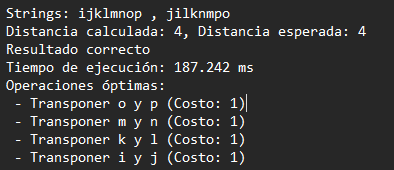
\includegraphics[width=0.45\textwidth]{images/trans-normal.png}%
            \label{fig:imagen1}
        }
        \hfill
        % Segunda imagen
        \subfloat[Transposiciones con costo modificado.]{%
            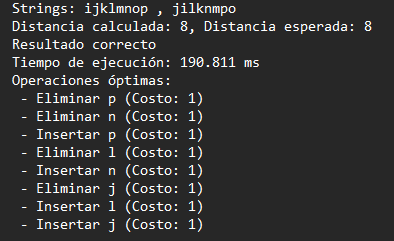
\includegraphics[width=0.45\textwidth]{images/trans-modificada.png}%
            \label{fig:imagen2}
        }
        \caption{Ejemplo ejecución de transposiciones.}
        \label{fig:trans}
    \end{figure}

    Por lo tanto, al modificar los costos de las operaciones, no
    se modifica en gran medida el tiempo de ejecución de los algoritmos
    al igual con el uso de memoria, pero si las operaciones las cuales producen la distancia de edición
    minima. Por lo tanto,
    se evidencia que los costos de de las operaciones no afectan a la complejidad
    temporal y espacial.

    \item Cadenas vacías y caracteres repetidos
    
        \begin{table}[H]
        \centering
        \begin{tabular}{|c|c|c|}
        \hline
        \textbf{Tipo/Data} & \textbf{Cadenas vacías} & \textbf{Caracteres repetidos}\\ \hline
        Fuerza Bruta (ms) & 0.0033952 & 183.942 \\ \hline
        Programación Dinámica (ms) & 0.0099436 & 0.0952444 \\ \hline
        Memoria FB (KB) & 97.15 & 106.5   \\ \hline
        Memoria PD (KB) & 100.7 & 143.9 \\ \hline
      
        \end{tabular}
        \caption{Tabla con valores de prueba para cadenas vacías y caracteres repetidos}
        \label{tab:tabla2}
        \end{table}

    
    Para el dataset de cadenas vacías podemos observar que al algoritmo
    de fuerza bruta le toma menos tiempo en resolver la consulta con
    respecto al de programación dinámica. Por otro lado, el uso de memoria
    es similar en los dos casos.

    Estos resultados se deben a las complejidades temporales y espaciales
    de cada algoritmo, para el algoritmo de fuerza bruta, su tiempo de ejecución
    es exponencial con respecto al tamaño mas pequeño de la entrada, 
    al tener una entrada con largo 0, el algoritmo resuelve el problema
    muy eficientemente, podríamos decir que le toma tiempo $4^0=1$.

    Por el lado del algoritmo de programación dinámica, su tiempo de ejecución
    se modela según los tamaños de las dos entradas mas 1, por lo tanto, podríamos
    decir que le toma tiempo $1*9=9$, lo cual es mayor que el algoritmo de
    fuerza bruta.

    Ademas, los usos de memoria son similares ya que el algoritmo de 
    programación dinámica basa su uso de memoria en los tamaños de las
    dos entradas, al tener
    una de las entradas pequeñas, el uso de memoria disminuye.

    Sobre el dataset de caracteres repetidos, podemos observar que
    el algoritmo de fuerza bruta es mas ineficiente con respecto 
    al de programación dinámica, no obstante, el uso de memoria
    es mayor en este ultimo.

    Con esto, podemos evidenciar en la practica que las complejidades
    temporales y espaciales para cada algoritmo se cumplen.

    
    \item Palabras aleatorias con matrices de costo estándar y modificado
    
        \begin{table}[H]
        \centering
        \begin{tabular}{|c|c|c|c|c|}
        \hline
        \textbf{Data/Tipo} & \textbf{Fuerza Bruta (ms)} & \textbf{Programación Dinámica (ms)} & \textbf{Memoria FB (KB)} & \textbf{Memoria PD (KB)} \\ \hline
        Menor a 2 & 0.00890745 & 0.0101063 & 97.55 & 98.02\\ \hline
        3 a 4 & 0.15021 & 0.0225789 & 99.37 &  104 \\ \hline
        7 & 33.0569 & 0.0653561 & 105.2 & 131.1 \\ \hline
        8 & 180.548 & 0.0875144 & 108.2 & 145.6 \\ \hline
        8 Modificado & 181.627 & 0.0992815 & 105.5 & 145.2\\ \hline
        12 & 172570 & 0.219571 & No medido & 252.5\\ \hline
        \end{tabular}
        \caption{Tabla con valores de prueba para cadenas aleatorias}
        \label{tab:tabla3}
        \end{table}

\end{enumerate}

























En esta sección, los resultados obtenidos, como las gráficas o tablas, deben estar respaldados por los datos generados durante la ejecución de sus programas. Es fundamental que, junto con el informe, se adjunten los archivos que contienen dichos datos para permitir su verificación. Además, se debe permitir y especficiar como obtener esos archivos desde una ejecución en otro computador (otra infraestructura para hacer lso experimentos).

\textbf{No es necesario automatizar la generación de las gráficas}, pero sí es imprescindible que se pueda confirmar que las visualizaciones presentadas son producto de los datos generados por sus algoritmos, aunque la trazabilidad de los datos hasta las visualizaciones es esencial para garantizar que su validez: describa cómo se generaron los datos, cómo se procesaron y cómo se visualizaron de manera que pueda ser replicado por quien lea su informe.

Agregue gráficas que muestren los resultados de sus experimentos. La cantidad de páginas es limitada, por lo tanto escoja las gráficas más representativas y que muestren de manera clara los resultados obtenidos. Esta elección es parte de lo que se evaluara en la sección de presentación de resultados. Referencie las figuras en el texto, describa lo que se observa en ellas y por qué son relevantes.

En la \cref{fig:scatterplot_1} se muestra un scatterplot hecho con \href{https://es.overleaf.com/learn/latex/TikZ_package}{TikZ} con el tamaño ideal cuando se incluyen dos figuras. Queda a criterio de usted el decidir qué figuras incluir.

\begin{figure}[H]
    \centering
    
\begin{tikzpicture}
    %\begin{loglogaxis}[
    %\begin{semilogxaxis}[ % Cambiar a semilogxaxis    
    \begin{axis}[
        xlabel={Número de Cudastreams },
        ylabel={Tiempo [ms]},
        grid=major,
        legend pos=north west,
        legend cell align={left},
        width=16cm,
        height=10cm, 
        xtick=data,
    ]
    \addplot[blue, only marks, mark=square*] coordinates {
        (2   , 14.229344)
        (4   , 13.435616 )
        (8   , 12.929280 )
        (12  , 12.628000 )
        (16  , 13.286176 )
        (20  , 13.873152 )
        (24  , 13.531168 )
        (28  , 14.116384 )
        (32  , 14.518528 )
        (36  , 14.448992 )
        (40  , 14.356640 )
        (44  , 15.226560 )
        (48  , 14.473888 )
        (52  , 15.066720 )
        (56  , 15.426560 )
        (60  , 15.380416 )
        (64  , 15.348064 )
    };
    \addlegendentry{GPU\_51 (1)}
    \addplot[red, only marks, mark=square*] coordinates {
        (2  , 12.799264 ) 
        (4  , 12.956192 )
        (8  , 13.371104 )
        (12 , 14.495616 )
        (16 , 14.783360 ) 
        (20 , 15.152672 ) 
        (24 , 15.475488 ) 
        (28 , 15.676416 ) 
        (32 , 15.948800 ) 
        (36 , 16.064129 ) 
        (40 , 15.904544 ) 
        (44 , 16.157921 ) 
        (48 , 16.444992 ) 
        (52 , 16.943169 ) 
        (56 , 16.894304 ) 
        (60 , 17.689600 ) 
        (64 , 17.559551 ) 
    };
    \addlegendentry{GPU\_6 (2)}
    \addplot[green, only marks, mark=square*] coordinates {
        (6, 17.607168) 
        (12, 12.159264) 
        (24, 12.239648) 
        (24, 12.169376) 
        (48, 12.490624) 
        (72, 14.081920) 
    };
    \addlegendentry{GPU\_7 (3)}
   
\end{axis}
%\end{semilogxaxis} % Cambiar a semilogxaxis
\end{tikzpicture}

    \caption{Ejemplo de scatterplot hecho con tikz. Tamaño ideal 1.}
    \label{fig:scatterplot_1}
\end{figure}


\begin{figure}[H]
    \centering
    \begin{minipage}[t]{0.5\textwidth}
    \begin{tikzpicture}[scale=0.7]
    %\begin{loglogaxis}[
    %\begin{semilogxaxis}[ % Cambiar a semilogxaxis    
    \begin{axis}[
        xlabel={\Large Meandistance [\AA] },
        ylabel={\Large Efree [eV]},
        %grid=major,
        legend pos=north east,
        legend cell align={left},
        %log basis x=10,
        %log basis y=10,
        %xmin=2, xmax=2^21,
        %ymin=0.1, ymax=100,
        width=10cm, % Ajusta el ancho de la gráfica
        height=10cm, % Ajusta la altura de la gráfica
        %xtick=data,
    ]
    \addplot[magenta , only marks, mark=square*, mark options={draw=black,line width = 1pt}, mark size=4pt] coordinates {
        %(7.112914 ,	-255.554964)
        (5.807670 ,	-255.571675)
        (2.903835 ,	-255.534455)
        (5.029590 ,	-255.564079)
        (4.106643 ,	-255.551738)       
        };
    \addlegendentry{cantmax = 0} 
    \addplot[cyan , only marks, mark=square*, mark options={draw=black,line width = 1pt}, mark size=4pt] coordinates {
        (7.112914 ,	-255.554964)   
        };
        \addlegendentry{cantmax = 1} 
\end{axis}
%\end{semilogxaxis} % Cambiar a semilogxaxis
\end{tikzpicture}
    \end{minipage}%
    \begin{minipage}[t]{0.5\textwidth}
    \begin{tikzpicture}[scale=0.7]
    %\begin{loglogaxis}[
    %\begin{semilogxaxis}[ % Cambiar a semilogxaxis    
    \begin{axis}[
        xlabel={\Large Meandistance [\AA] },
        ylabel={\Large Efree [eV]},
        %grid=major,
        legend pos=north east,
        legend cell align={left},
        %log basis x=10,
        %log basis y=10,
        %xmin=2, xmax=2^21,
        %ymin=0.1, ymax=100,
        width=10cm, % Ajusta el ancho de la gráfica
        height=10cm, % Ajusta la altura de la gráfica
        %xtick=data,
    ]
    \addplot[magenta , only marks, mark=square*, mark options={draw=black,line width = 1pt}, mark size=4pt] coordinates {
        (4.845001   ,	-267.121023)	% 0
        (5.000617   ,	-267.145714)	% 0
        (4.760055   ,	-267.112360)	% 0
        (3.236691   ,	-266.851158)	% 0
        (3.356972   ,	-266.882713)	% 0
        %(5.427886   ,	-267.150822)	% 1
        (4.830514   ,	-267.115114)	% 0
        (3.144397   ,	-266.841800)	% 0
        %(4.280839   ,	-266.992946)	% 1
        (3.874418   ,	-266.969850)	% 0
        %(4.595953   ,	-267.006159)	% 2
        %(3.962469   ,	-266.940902)	% 1       
        };
    \addlegendentry{cantmax = 0} 
    \addplot[cyan , only marks, mark=square*, mark options={draw=black,line width = 1pt}, mark size=4pt] coordinates {
        (5.427886   ,	-267.150822)	% 1
        (4.280839   ,	-266.992946)	% 1
        (3.962469   ,	-266.940902)	% 1
        };
        \addlegendentry{cantmax = 1} 
    \addplot[orange , only marks, mark=square*, mark options={draw=black,line width = 1pt}, mark size=4pt] coordinates {
        (4.595953   ,	-267.006159)	% 2
        };
        \addlegendentry{cantmax = 2}
\end{axis}
%\end{semilogxaxis} % Cambiar a semilogxaxis
\end{tikzpicture}
    \end{minipage}%
    \caption{Ejemplo de scatterplot hecho con tikz. Tamaño ideal 2.}
    \label{fig:scatterplot_2}
\end{figure}

\begin{figure}[H]
    \centering
    \begin{minipage}[t]{0.5\textwidth}
        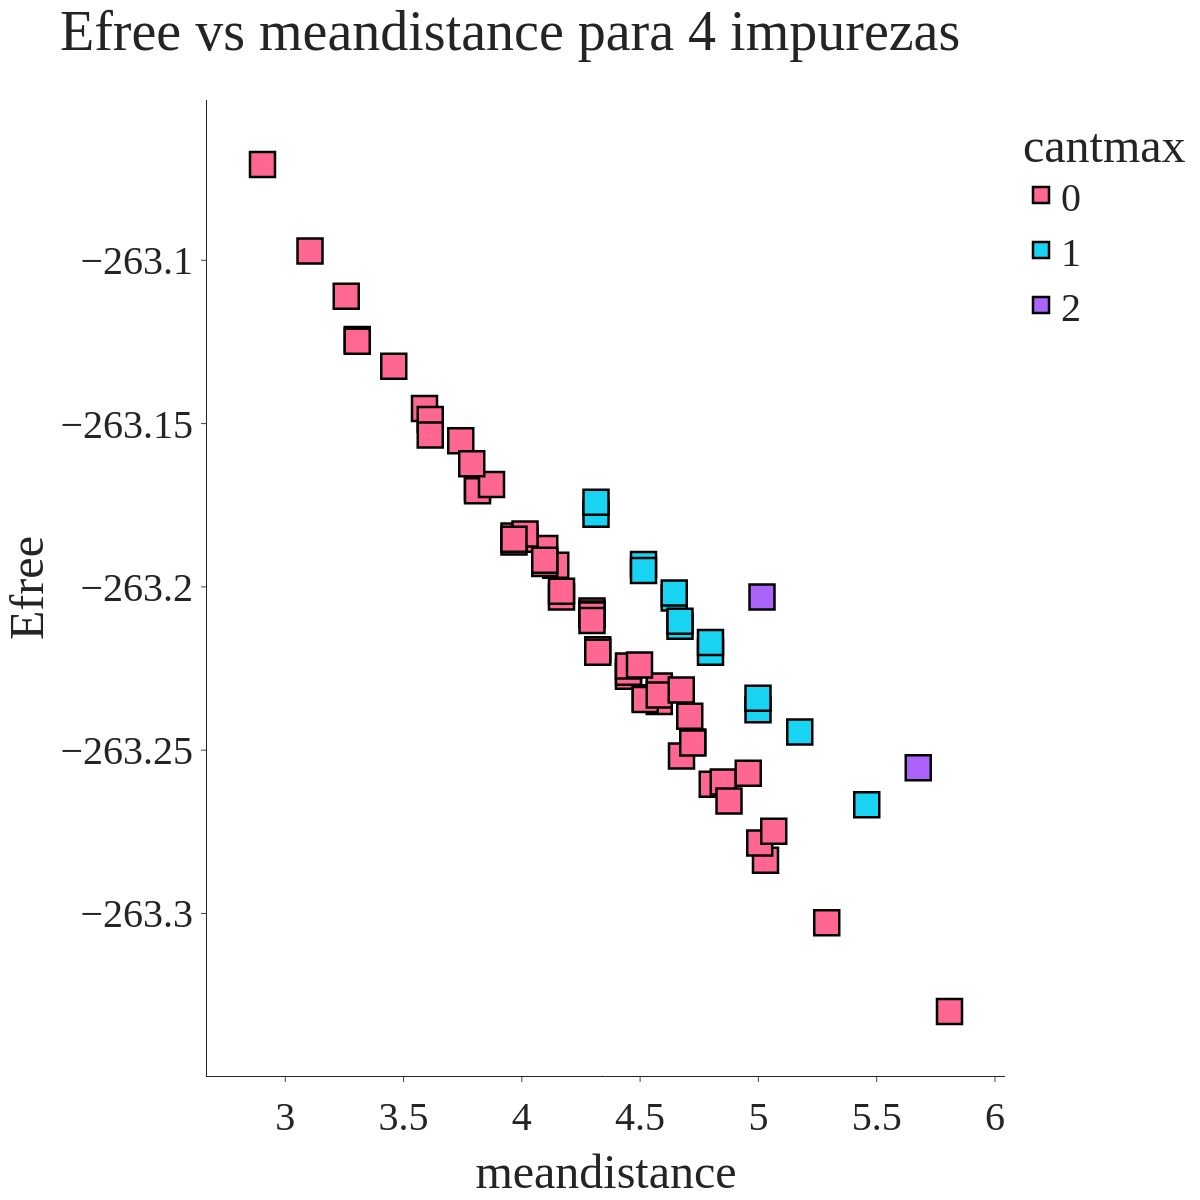
\includegraphics[width=\textwidth]{images/4_impurezas_cantmax_size10.png}
    \end{minipage}%
    \begin{minipage}[t]{0.5\textwidth}
        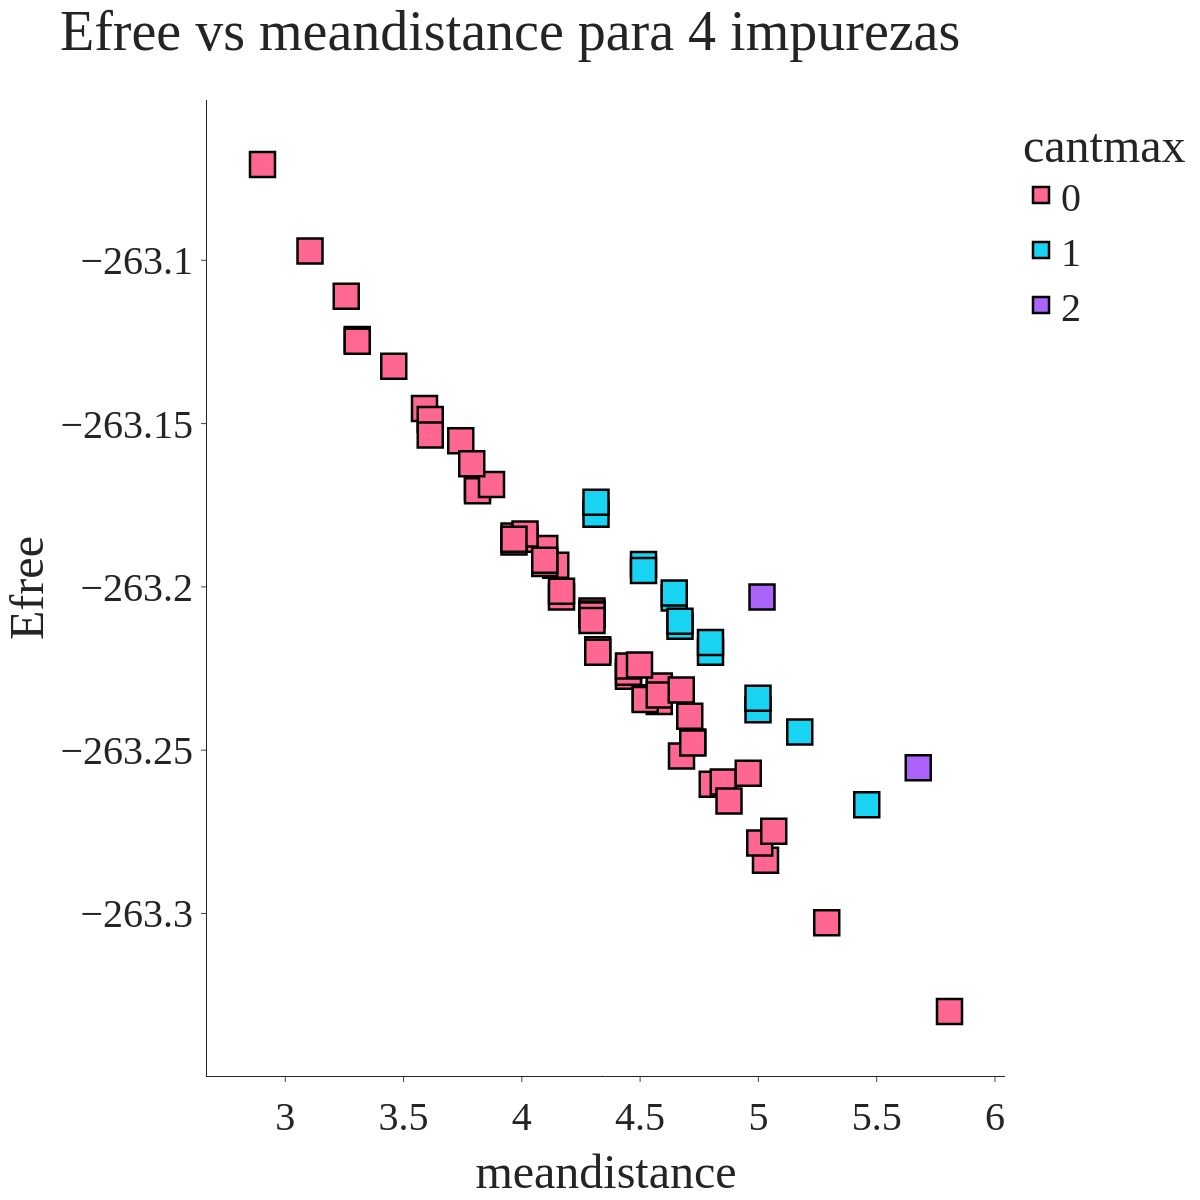
\includegraphics[width=\textwidth]{images/4_impurezas_cantmax_size10.png}    \end{minipage}%
    \caption{Ejemplo de scatterplot hecho con matplotlib.}
    \label{fig:scatterplot_3}
\end{figure}





\begin{mdframed}
    Recuerde que es imprescindible que se pueda replicar la generación de las gráficas, por lo que usted debe incluir cómo generó esos datos y  cómo podría generarlos la persona que revisa su entrega y ejecuta sus programas. Por ejemplo, si genera un scatterpolot con Tikz, usted debe explicar cómo obtener la tupla de valores que se usaron para generar la gráfica.
\end{mdframed}



\newpage
\section{Conclusiones}


El análisis e implementación del algoritmo de distancia de 
edición extendida, mediante las técnicas de fuerza bruta y
programación dinámica, permitieron validar empíricamente lo descrito
por la teoría en base a sus complejidades temporales y espaciales. 
Los resultados demuestran que, mientras el algoritmo basado en 
programación dinámica sobresale en términos de eficiencia temporal,
el uso de memoria aumenta a medida que crece la entrada. Por otra lado,
el algoritmo basado en fuerza bruta 
presenta un desempeño adecuado solo en entradas de tamaño reducido, a 
medida que crece la entrada, la eficiencia de este algoritmo empeora,
pero su uso de memoria se comporta de manera lineal.

Este reporte no solo confirma que la programación dinámica 
es más adecuada para entradas más grandes, sino que también
evidencia cómo la elección del algoritmo depende del contexto, 
ya que el bajo uso de memoria del algoritmo de fuerza bruta podría
ser un factor clave.
Por otro lado, los costos variables sobre la secuencia
de operaciones óptimas no represento un cambio en los tiempos
de ejecución o uso de memoria, reafirmando que estos parámetros 
no afectan a las complejidades, pero sí al comportamiento del algoritmo.  

En resumen, el trabajo logra comparar exitosamente 
las distintas técnicas de diseño de algoritmos, 
comprobando empíricamente la teoría, asi, se puede 
seguir desarrollando en base a lo propuesto para mejorar
estas técnicas.














\begin{comment}

\begin{mdframed}
    \textbf{La extensión máxima para esta sección es de 1 página.}
\end{mdframed}

La conclusión de su informe debe enfocarse en el resultado más importante de su trabajo. No se trata de repetir los puntos ya mencionados en el cuerpo del informe, sino de interpretar sus hallazgos desde un nivel más abstracto. En lugar de describir nuevamente lo que hizo, muestre cómo sus resultados responden a la necesidad planteada en la introducción.

\begin{itemize}
    \item  No vuelva a describir lo que ya explicó en el desarrollo del informe. En cambio, interprete sus resultados a un nivel superior, mostrando su relevancia y significado.
    \item Aunque no debe repetir la introducción, la conclusión debe mostrar hasta qué punto logró abordar el problema o necesidad planteada en el inicio. Reflexione sobre el éxito de su análisis o experimento en relación con los objetivos propuestos.
    \item No es necesario restablecer todo lo que hizo (ya lo ha explicado en las secciones anteriores). En su lugar, centre la conclusión en lo que significan sus resultados y cómo contribuyen al entendimiento del problema o tema abordado.
    \item No deben centrarse en sí mismos o en lo que hicieron durante el trabajo (por ejemplo, evitando frases como "primero hicimos esto, luego esto otro...").
    \item Lo más importante es que no se incluyan conclusiones que no se deriven directamente de los resultados obtenidos. Cada afirmación en la conclusión debe estar respaldada por el análisis o los datos presentados. Se debe evitar extraer conclusiones generales o excesivamente amplias que no puedan justificarse con los experimentos realizados.
\end{itemize}

\end{comment}

\newpage

\section{Condiciones de entrega}
% Condiciones generales de tareas de Algoritmos y Complejidad, 20231
  \begin{itemize}
  \item
    La tarea se realizará \tca{individualmente}
    (esto es grupos de una persona),
    sin excepciones.
  \item
    La entrega debe realizarse vía \url{http://aula.usm.cl}
    en un \tca{tarball} en el área designada al efecto,
    en el formato \tca{\texttt{tarea-\tnum-{rol}.tar.gz}}
    (\texttt{rol} con dígito verificador y sin guión).

    Dicho \tca{tarball} debe contener las fuentes en \LaTeXe{}
    (al menos \tca{\texttt{tarea-\tnum.tex}})
    de la parte escrita de su entrega,
    además de un archivo \tca{\texttt{tarea-\tnum.pdf}},
    correspondiente a la compilación de esas fuentes.
  \item Si se utiliza algún código, idea, o contenido extraído de otra fuente, este \textbf{debe} ser citado en el lugar exacto donde se utilice, en lugar de mencionarlo al final del informe. 
  \item
    Asegúrese que todas sus entregas tengan sus datos completos:
    número de la tarea, ramo, semestre, nombre y rol.
    Puede incluirlas como comentarios en sus fuentes \LaTeX{}
    (en \TeX{} comentarios son desde \% hasta el final de la línea)
    o en posibles programas.
    Anótese como autor de los textos.
 
  \item
    Si usa material adicional al discutido en clases,
    detállelo.
    Agregue información suficiente para ubicar ese material
    (en caso de no tratarse de discusiones con compañeros de curso
     u otras personas).
  \item No modifique \texttt{preamble.tex}, \texttt{tarea\_main.tex}, \texttt{condiciones.tex}, estructura de directorios, nombres de archivos, configuración del documento, etc. Sólo agregue texto, imágenes, tablas, código, etc. En el códigos funte de su informe, no agregue paquetes, ni archivos .tex (a excepción de que agregue archivos en \texttt{/tikz}, donde puede agregar archivos .tex con las fuentes de gráficos en \texttt{TikZ}).

\ifprograms
  \item
    Su programa ejecutable debe llamarse \tca{\texttt{tarea\tnum}},
    de haber varias preguntas solicitando programas,
    estos deben llamarse usando el número de la pregunta,
    como \tca{\texttt{tarea\tnum-1}},
    \tca{\texttt{tarea\tnum-2}},
    etc.
    Si hay programas compilados, con en este caso,
    incluya una \tca{\texttt{Makefile}}
    que efectúe las compilaciones correspondientes.

    Los programas se evalúan según que tan claros
    (bien escritos)
    son, si se compilan y ejecutan sin errores o advertencias según corresponda.
    Parte del puntaje es por ejecución correcta con casos de prueba.
    Si el programa no se ciñe a los requerimientos de entrada y salida,
    la nota respectiva es cero.
\fi    
  \item
    %La entrega debe realizarse dentro del plazo indicado en \url{http://aula.usm.cl}:
    La fecha límite de entrega es el día \tca{10 de noviembre de 2024}.

    \begin{center}
        \Large{
          \textbf{NO SE ACEPTARÁN TAREAS FUERA DE PLAZO}.
        }
        \normalsize
    \end{center}
     
    
  \item
    Nos reservamos el derecho de llamar a interrogación
    sobre algunas de las tareas entregadas.
    En tal caso,
    la nota de la tarea será la obtenida en la interrogación.
    \begin{center}
      \Large{
        \textbf{NO PRESENTARSE A UN LLAMADO A INTERROGACIÓN SIN JUSTIFICACIÓN PREVIA SIGNIFICA AUTOMÁTICAMENTE NOTA 0.}
      }
    \end{center}
    
  \end{itemize}

%%% Local Variables:
%%% mode: latex
%%% ispell-local-dictionary: "spanish"
%%% End:

  
% LocalWords:  tarball tar gz pdf min entregable Makefile puntaje
% LocalWords:  Moodle

\newpage
\appendix


\section{Apéndice 1}

Los gráficos de uso de memoria generados por massif se encuentran aquí \cite{Experimentos}
\printbibliography

\end{document}


